
\documentclass[12pt,ngerman,a4paper]{scrartcl}

\usepackage{babel}


\usepackage[utf8]{inputenc}
\usepackage[T1]{fontenc}
\usepackage{lmodern}

\usepackage{amsmath,amssymb,amsfonts,amsthm}

\usepackage{graphicx}

\usepackage{titlesec}
\titleformat*{\section}{\Large\bfseries}

\usepackage[a4paper,left=2.5cm,right=2.5cm,top=2.5cm,bottom=2.5cm]{geometry}

\begin{document}
\section{\hspace{3mm}Die Normalverteilung}
Die Normalverteilung, auch Gauß-Verteilung genannt, ist eine der wichtigsten Wahrscheinlichkeitsverteilungen. Die Dichtefunktion
\begin{align}
 \mathcal{N}(x, \sigma, \mu) = \frac{1}{\sqrt{2\pi \sigma^2}} \exp \left(-\frac{(x-\mu)^2}{2\sigma^2}\right) 
 \label{ga}
 \end{align} wird mit dem Erwartungswert $\mu \in \mathbb{R}$ und der Varianz $\sigma^2$ > 0 parametrisiert. In Abbildung \ref{Abb} wird die Gauß-Verteilung aus Gleichung \eqref{ga} im Intervall $x \in [-5, 5]$ für die Parameterpaare \[(\mu, \sigma) \in \{(0,0.2), (0,1), (0,5), (-2, 0.5)\}\] dargestellt.\\
 
\begin{figure}[h!]
\begin{center}
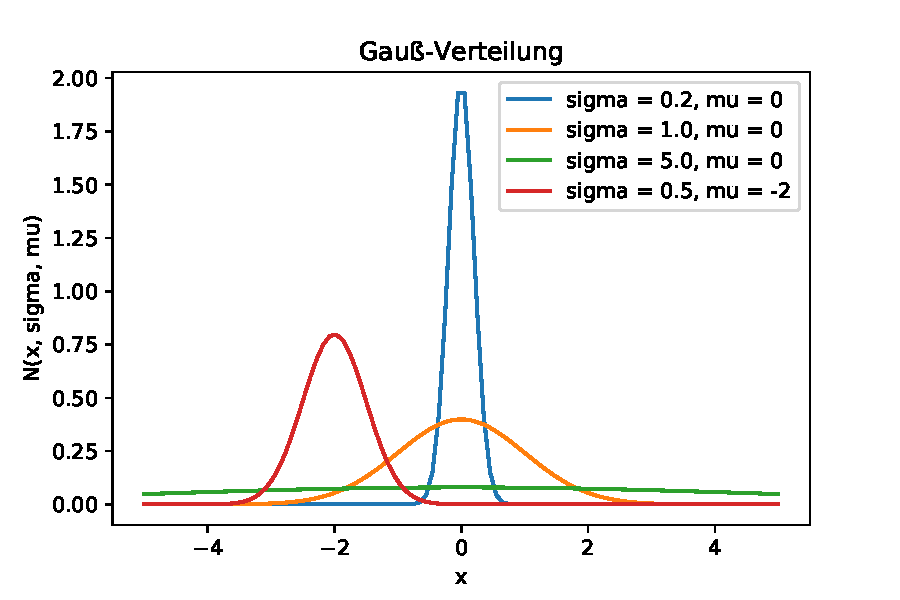
\includegraphics[width=0.7\textwidth]{1.pdf}
\caption{Die Normalverteilung aus \eqref{ga} für $(\mu, \sigma) \in \{(0,0.2), (0,1), (0,5), (-2, 0.5)\}$}
\label{Abb}
\end{center}
\end{figure}
\end{document}